%Example of use of oxmathproblems latex class for problem sheets
\documentclass{oxmathproblems}
\usepackage{tikz}
\usepackage{algorithmic}
\usepackage{algorithm,float}
\usepackage{hyperref}
\hypersetup{hidelinks,
  colorlinks=true,
  allcolors=black,
  pdfstartview=Fit,
  breaklinks=true}
\usepackage{amsmath}  % 这个包提供了数学环境和命令

%(un)comment this line to enable/disable output of any solutions in the file
%\printanswers

%define the page header/title info
\course{Algorithm Design and Analysis (Fall 2023)}
\sheettitle{Assignment 5\\Deadline: Jan 2, 2023\\\small{Yuqing Tu 522030910152}} %can leave out if no title per sheet

\makeatletter
\newenvironment{breakablealgorithm}
  {% \begin{breakablealgorithm}
  \begin{center}
    \refstepcounter{algorithm}% New algorithm
    \hrule height.8pt depth0pt \kern2pt% \@fs@pre for \@fs@ruled 画线
    \renewcommand{\caption}[2][\relax]{% Make a new \caption
    {\raggedright\textbf{\ALG@name~\thealgorithm} ##2\par}%
    \ifx\relax##1\relax % #1 is \relax
      \addcontentsline{loa}{algorithm}{\protect\numberline{\thealgorithm}##2}%
    \else % #1 is not \relax
      \addcontentsline{loa}{algorithm}{\protect\numberline{\thealgorithm}##1}%
    \fi
    \kern2pt\hrule\kern2pt
    }
  }{% \end{breakablealgorithm}
    \kern2pt\hrule\relax% \@fs@post for \@fs@ruled 画线
  \end{center}
  }
\makeatother

\begin{document}
\begin{questions}

\miquestion[30] \textbf{[Menger's Theorem]}
Let $G=(V,E)$ be a connected undirected graph. The \emph{edge connectivity} of $s,t\in V$ is the minimum number of edges whose removal disconnects $s$ and $t$.
The \emph{vertex connectivity} of $s,t$ is the minimum number of graph elements (any vertex in $V\setminus\{s,t\}$ or any edge in $E$) whose removal disconnects $s$ and $t$. Menger's Theorem states that the edge connectivity of $s,t$ is exactly the number of edge-disjoint paths between $s$ and $t$ and the vertex connectivity of $s,t$ is exactly the number of \emph{internally} vertex-disjoint paths between $s$ and $t$. (Obviously, two paths between $s$ and $t$ are not vertex-disjoint since they intersect at $s$ and $t$; \emph{internally} vertex disjoint means they are disjoint except for $s$ and $t$.)

Prove that Menger's Theorem is just a consequence of the max-flow-min-cut theorem. Be sure the network you construct is \emph{directed} and \emph{capacitated}.

\textbf{Solution:}

\begin{parts}
\part Prove that the edge connectivity of $s,t$ is exactly the number of edge-disjoint paths between $s$ and $t$:\\
Let $G' = (V, E')$ be a directed graph and $E' = \{\langle u, v\rangle, \langle v, u\rangle \vert \forall u, v \in V\}$. The capacity of $G'$'s all edges is $1$.
\begin{itemize}
\item[1)] First, we prove that the number of edge-disjoint paths $n$ between $s$ and $t$ is equal to the max-flow $f$ in $G'$ from $s$ to $t$:\\
Because each edge's capacity is $1$, so there are $f$ paths in $G'$ that contribute $1$ to the max-flow. And in these paths, no two paths share the same edge. Otherwise, the capacity of the shared edge will overflow. Therefore, there are $f$ edge-disjoint paths between $s$ and $t$, which means $n = f$.
\item[2)] Then, we prove that the edge connectivity of $s,t$ is equal to the min-cut between $s$ and $t$:\\
Because each edge's capacity is $1$, so the min-cut is equal to the number of the edges in the min-cut. According to the definition, it is obviously that the edge connectivity of $s,t$ is equal to the min-cut between $s$ and $t$.
\end{itemize}
So we have proved that a part of Menger's Theorem is just a consequence of the max-flow-min-cut theorem.
\part Prove that the vertex connectivity of $s,t$ is exactly the number of internally vertex-disjoint paths between $s$ and $t$:\\
Let $G'' = (V, E')'$ be a directed graph. In $G''$, make each vertex $u \in V$ into ``big vertex'' as shown below.
\begin{figure}[H]
  \centering
  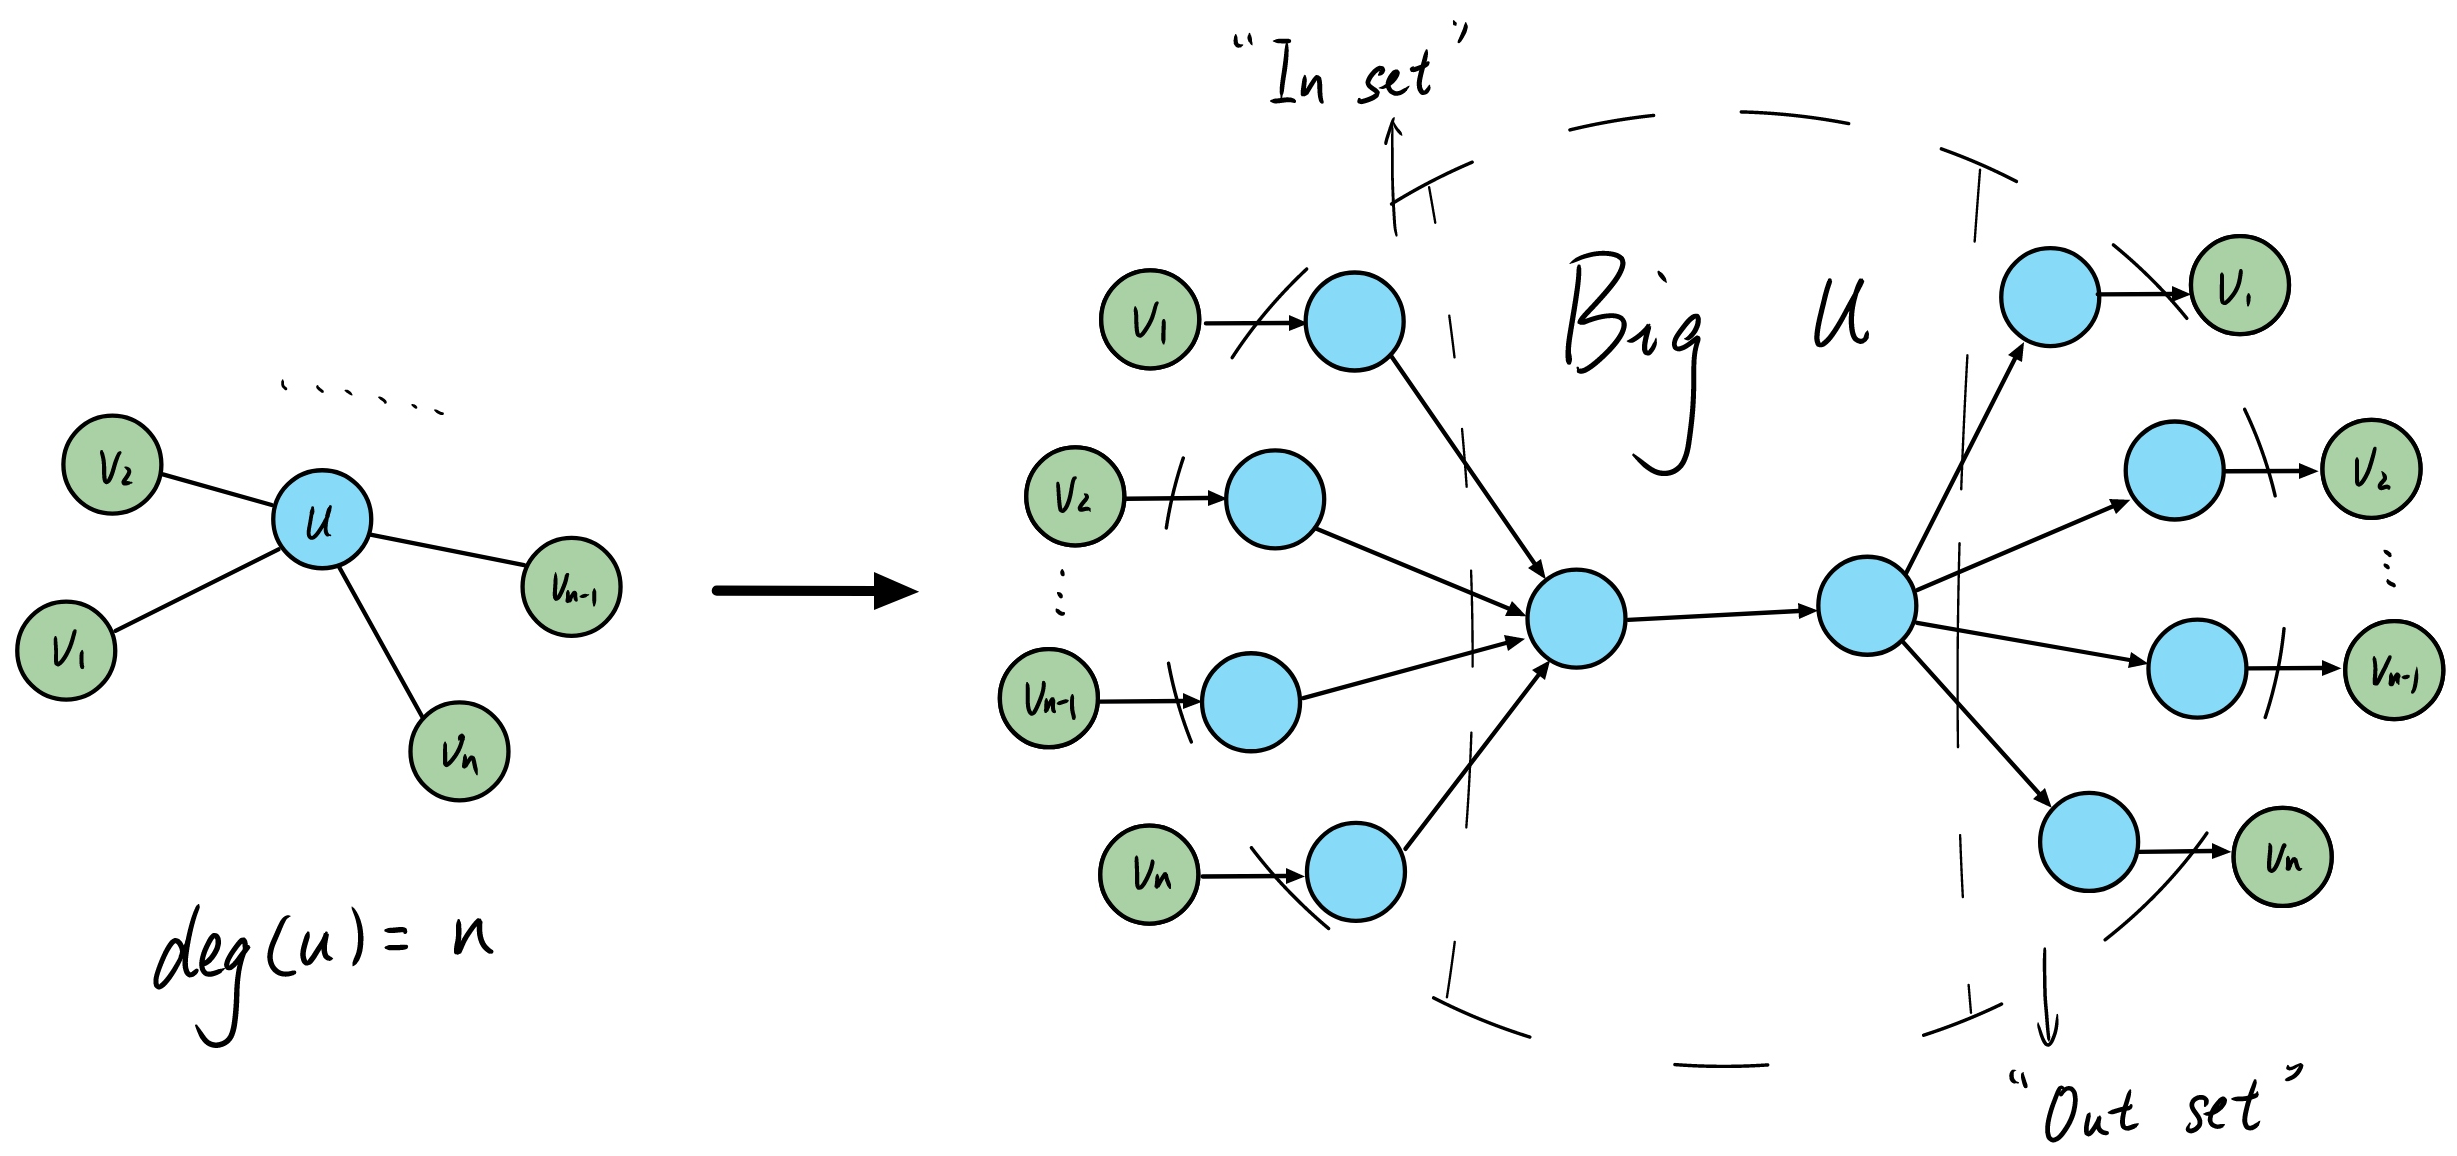
\includegraphics[width=\textwidth]{A5G1.png}
\end{figure}
And between $u, v \in V$, $u$'s outgoing edges will reach to the vertex in ``In set'' of ``big $v$'' and $u$'s incoming edges will reach to the vertex in ``Out set'' of ``big $v$''. The capacity of $G''$'s all edges is $1$. So the maximum capacity of each ``big vertex'' is $1$.
\begin{itemize}
\item[1)] First, we prove that the number of internally vertex-disjoint paths $n$ between $s$ and $t$ is equal to the max-flow $f$ in $G'$ from $s$ to $t$:\\
Because each edge's capacity is $1$, so there are $f$ paths in $G'$ that contribute $1$ to the max-flow. And in these paths, no two paths share the same vertex. Otherwise, the capacity of the shared vertex will overflow. Therefore, there are $f$ vertex-disjoint paths between $s$ and $t$, which means $n = f$.
\item[2)] Then, we prove that the vertex connectivity of $s,t$ is equal to the min-cut between $s$ and $t$:\\
Because each edge's capacity is $1$ and the maximum capacity of each ``big vertex'' is $1$, so the min-cut is equal to the number of the edges and ``big vertices'' in the min-cut. According to the definition, it is obviously that the vertex connectivity of $s,t$ is equal to the min-cut between $s$ and $t$.
\end{itemize}
So the other part Menger's Theorem is just a consequence of the max-flow-min-cut theorem.
\end{parts}
To sum up, Menger's Theorem is just a consequence of the max-flow-min-cut theorem.

\miquestion[30] \textbf{[Perfect Matching on Bipartite Graph]}
A graph is \emph{regular} if every vertex has the same degree.
Let $G=(A,B,E)$ be a regular bipartite graph with $|E|>0$.
\begin{parts}
\part[10] Prove that $|A|=|B|$.
\part[15] Let $n=|A|=|B|$. Can we conclude that $G$ must contain a matching of size $n$? If so, prove it; if not, provide a counterexample.
\end{parts}

\textbf{Proof:}
\begin{parts}
\part In a bipartite graph, we have $\sum_{u\in A}deg(u) = \sum_{v\in B}deg(v)$. It is because that the end vertices $u, v$ of every edge $e$ in $G$ can't both in $A$ or $B$. So each edge will contribute 1 to both $A$'s sum of degree and $B$'s sum of degree. And because every vertex has the same degree $k$, so
$$\frac{\sum_{u\in A}deg(u)}{k} = \frac{\sum_{v\in B}deg(v)}{k}$$
$$|A|=|B|$$
\part Yes, we can!\\
Let
$$G' = (V, E')$$
$$V = A + B + \{s, t\}$$
$$E' = \{\langle s, u\rangle |\forall u \in A\} + \{\langle v, t\rangle |\forall v \in B\} + \{\langle u, v\rangle |\forall u \in A, \forall v \in B\}$$
The capacity of $e_1\in \{\langle s, u\rangle |\forall u \in A\} + \{\langle v, t\rangle |\forall v \in B\}$ is $1$ and the capacity of $e_2\in \{\langle u, v\rangle |\forall u \in A, \forall v \in B\}$ is $\infty$.\\
To prove it, we just need to prove that the max-flow from $s$ to $t$ of $G'$ is $n$.\\
For every vertex $u\in A$, it gets a input flow of size $1$ from $s$. And we divide it into $k$ output flows of size $\frac{1}{k}$. Each output flow $f_i$ will be the input of $v_i\in B$. So for every vertex $v \in B$, it gets $k$ input flows of size $\frac{1}{k}$, then there will be a output flow of size $1$ from $v$ to $t$. Finally, $t$ will get $n$ input flows of size $1$, so the flow from $s$ to $t$ is $n$. And we know that the flow's upper bound from $s$ to $t$ is $n$, so the max-flow from $s$ to $t$ of $G'$ is $n$. Then the proposition is proved.
\end{parts}

\miquestion[40]\textbf{[K\"{o}nig-Egerv\'{a}ry Theorem]}
In the class, we have seen that the maximum matching problem can be formulated by the following linear program
\begin{align*}
\text{maximize }& \sum_{e\in E}x_e \\
\text{subject to }&\sum_{e:e=(u,v)}x_e\leq 1  \tag{$\forall v\in V$}\\
&x_e\geq0\tag{$\forall e\in E$}
\end{align*}
and the minimum vertex cover problem can be formulated by the following linear program
\begin{align*}
\text{minimize }& \sum_{u\in V}x_u \\
\text{subject to }&x_u+x_v\geq 1  \tag{$\forall (u,v)\in E$}\\
&x_u\geq0\tag{$\forall u\in V$}
\end{align*}
We have also seen that the second linear program is the dual program of the first.
\begin{parts}
\part[20] Prove that both linear programs have integral optimal solutions if the graph is bipartite.
\part[10] Using the result in the first part, prove K\"{o}nig-Egerv\'{a}ry Theorem, which states that the size of the maximum matching equals to the size of the minimum vertex cover in a bipartite graph.
\part[10] Provide a counterexample showing that the claim fails for non-bipartite graphs.
\end{parts}

\textbf{Solution:}
\begin{parts}
\part The primal linear program can be expressed as
\begin{align*}
  \text{maximize }& c^Tx_e \\
  \text{subject to }&Ax_e\leq b  \notag\\
  &x_e\succcurlyeq 0 \notag
\end{align*}
and the dual program can be expressed as
\begin{align*}
  \text{maximize }& b^Tx_v \\
  \text{subject to }&A^Tx_v\leq c  \notag\\
  &x_v\succcurlyeq 0 \notag
\end{align*}
Where
\begin{equation}
  \mathbf{A} = 
  \begin{bmatrix}
      a_{11} & a_{12} & \cdots & a_{1|E|} \\
      a_{21} & a_{22} & \cdots & a_{2|E|} \\
      \cdots & \cdots & \cdots & \cdots \\
      a_{|V|1} & a_{|V|2} & \cdots & a_{|V||E|} \notag
  \end{bmatrix}
\end{equation}
(if the vertex $i$ is one of the end of edge $j$, $a_{ij} = 1$, else $a_{ij} = 0$), $b = [1\ 1\ \cdots \ 1]$ has columns $|v|$, $c = [1\ 1\ \cdots \ 1]$ has columns $|E|$, $x_e = [x_{e1}\ x_{e1}\ \cdots \ x_{e|E|}]$ and $x_v = [x_{v1}\ x_{v2}\ \cdots \ x_{v|V|}]$.\\
To prove both linear programs have integral optimal solutions, we just need to prove $A$ is a totally unimodular matrix.\\
Prove by induction:
\begin{itemize}
  \item Base Step: Each cell of $a$ belongs to $\{0, 1\}$
  \item Inductive Step: Suppose every $k \times k$ submatrix of $A$ has determinant belongs to $\{0, -1, 1\}$. Consider any $(k+1) \times (k+1)$ submatrix $A'$
  \item Case 1: If a column of $A'$ is all-zero, then $det(Z') = 0$
  \item Case 2: If a column of $A'$ contains only one $1$ entry, then $det(A') = \pm 1$ times the determinant of a $k\times k$ submatrix. $det(A') \in \{0, -1, 1\}$ by induction hypothesis
  \item Case 3: If every column of $A'$ has two $1$ entries, then $k+1$ must be an even number. It is because if the subgraph of this bipartite graph is a cycle, it must an even cycle. Assume $c_1, c_2, \cdots, c_{k+1}$ is all the columns of $A'$ that their order is the order in which they are traversed through the even cycle(each column corresponds to an edge). It is obviously that $\sum_{i=1}^{k+1}(-1)^ic_i$ is a zero vector. So $det(A') = 0$
  \item So the determinant of any submatrix of $A$ belongs to $\{0, -1, 1\}$, which means $A$ is a totally unimodular matrix.
\end{itemize}
So both linear programs have integral optimal solutions.

\part Because both linear programs have integral optimal solutions if the graph is bipartite, so we can solve linear programs in order to get the size of the maximum matching and the size of the minimum vertex cover in a bipartite graph. Then by Strong Duality Theorem, $Primal\ OPT = Dual\ OPT$, so the size of the maximum matching equals to the size of the minimum vertex cover in a bipartite graph.

\part
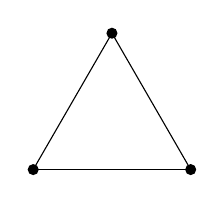
\begin{tikzpicture}
  \draw (0,0) -- (1,1.732);
  \draw (1,1.732) -- (2,0);
  \draw (0,0) -- (2,0);
  \fill (0,0) circle (2pt);
  \fill (1,1.732) circle (2pt);
  \fill (2,0) circle (2pt);
\end{tikzpicture}
\end{parts}

\miquestion[Bonus 60]
\textbf{[Dinic's Algorithm]}
In this question, we are going to work out \emph{Dinic's algorithm} for computing a maximum flow.
Similar to Edmonds-Karp algorithm, in each iteration of Dinic's algorithm, we update the flow $f$ by increasing its value and then update the residual network $G^f$.
However, in Dinic's algorithm, we push flow along \emph{multiple} $s$-$t$ paths in the residual network instead of a \emph{single} $s$-$t$ path as it is in Edmonds-Karp algorithm.

In each iteration of the algorithm, we find the \emph{level graph} of the residual network $G^f$.
Given a graph $G$ with a source vertex $s$, its level graph $\overline{G}$ is defined by removing edges from $G$ such that only edges pointing from level $i$ to level $i+1$ are kept, where vertices at level $i$ are those vertices at distance $i$ from the source $s$.
An example of level graph is shown in Fig.~\ref{fig:levelgraph}.

Next, the algorithm finds a \emph{blocking flow} on the level graph $\overline{G}^f$ of the residual network $G^f$.
A blocking flow $f$ in $G$ is a flow such that each $s$-$t$ path contains at least one \emph{critical edge}.
Recall that an edge $e$ is \emph{critical} if the amount of flow on it reaches its capacity: $f(e)=c(e)$.
Fig.~\ref{fig:blockingflow} gives examples for blocking flow.

Dinic's algorithm is then described as follows.
\begin{enumerate}
    \item Initialize $f$ to be the empty flow, and $G^f=G$.
    \item Do the following until there is no $s$-$t$ path in $G^f$:
    \begin{itemize}
        \item construct the level graph $\overline{G}^f$ of $G^f$.
        \item find a blocking flow on $\overline{G}^f$.
        \item Update $f$ by adding the blocking flow to it, and update $G^f$.
    \end{itemize}
\end{enumerate}

Complete the analysis of Dinic's algorithm by solving the following questions.
\begin{parts}
\part[15] Prove that, after each iteration of Dinic's algorithm, the distance from $s$ to $t$ in $G^f$ is increased by at least $1$.
\part[15] Design an $O(|V|\cdot |E|)$ time algorithm to compute a blocking flow on a level graph.
\part[10] Show that the overall time complexity for Dinic's algorithm is $O(|V|^2\cdot|E|)$.
\part[20] \textbf{(challenging)} We have seen in the class that the problem of finding a maximum matching on a bipartite graph can be converted to the maximum flow problem. Show that Dinic's algorithm applied to finding a maximum matching on a bipartite graph only requires time complexity $O(|E|\cdot\sqrt{|V|})$.
\end{parts}

\begin{figure}[H]
    \centering
    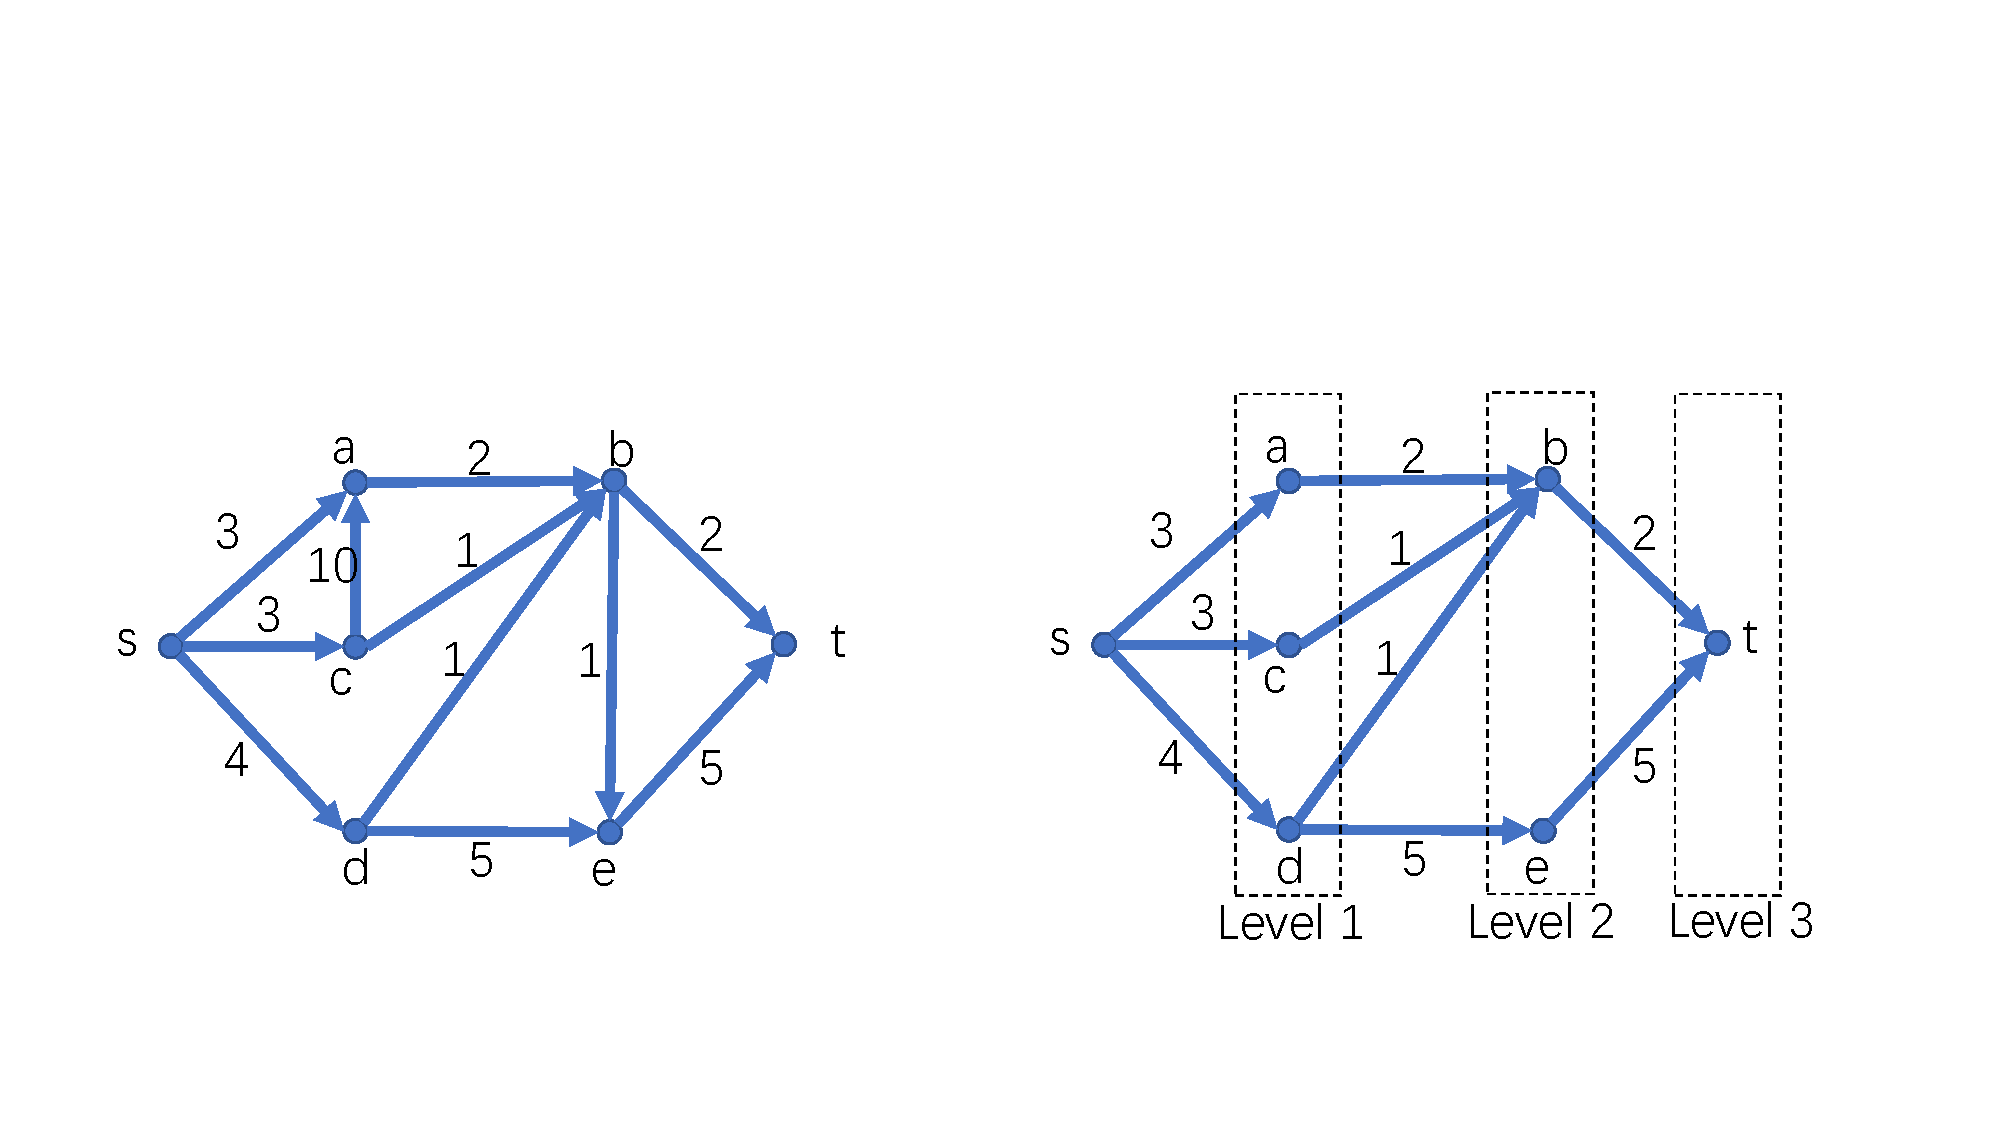
\includegraphics[width=\textwidth]{levelgraph.pdf}
    \caption{The graph shown on the right-hand side is the level graph of the graph on the left-hand side. Only edges pointing to the next levels are kept. For example, the edges $(c,a)$ and $(b,e)$ are removed, as they point at vertices at the same level. If there were edges pointing at previous levels, they should also be removed.}
    \label{fig:levelgraph}
\end{figure}

\begin{figure}[H]
    \centering
    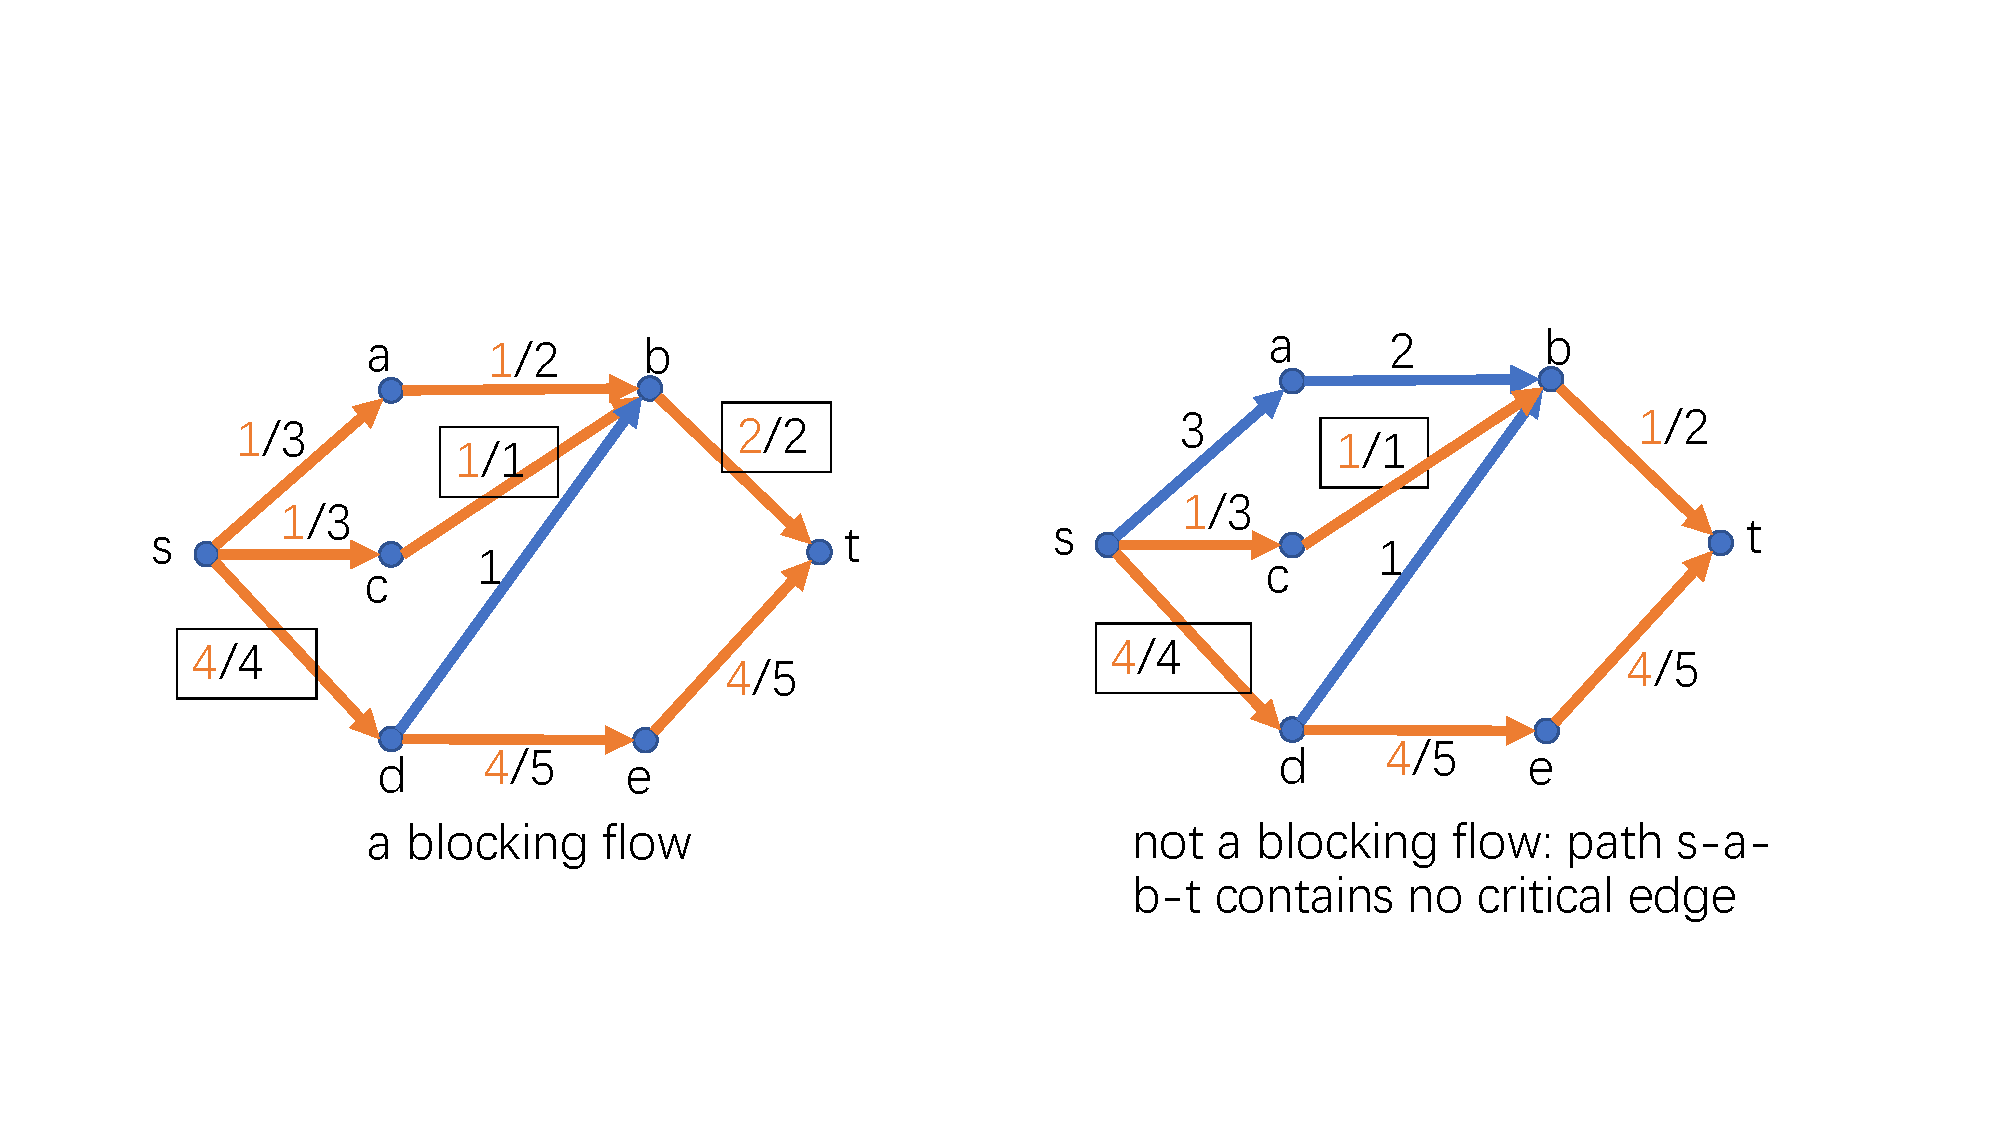
\includegraphics[width=\textwidth]{blockingflow.pdf}
    \caption{Blocking flow examples}
    \label{fig:blockingflow}
\end{figure}

\textbf{Solution:}

\begin{parts}
  \part Assume that in this iteration, the distance from $s$ to $t$ is $n$. Because in each iteration, we find a blocking flow on $\overline{G}^f$, which means that each $s$-$t$ path contains at least one critical edge. So when we update $G^f$, these $s$-$t$ path will no longer exist. In next iteration, if
  \begin{enumerate}
    \item there is no $s$-$t$ path on $\overline{G}^f$, then the distance from $s$ to $t$ is $\infty$, obviously increasing more than $1$.
    \item there is some new $s$-$t$ path on $\overline{G}^f$, then these paths' distance mustn't be $n$ because all $s$-$t$ paths with $n$ distance were eliminated in the last update. These paths' distance are also not smaller than $n$ because in the last update, each new edge is added from high level to low level, so these new edges won't do any help to reduce the distance from $s$ to $t$. To sum up, the the distance from $s$ to $t$ must be bigger than $n$ and it is an integer, so the distance from $s$ to $t$ is increased by at least $1$.
  \end{enumerate}
  In conclusion, the distance from $s$ to $t$ in $G^f$ is increased by at least $1$.\\
  \part 
  \begin{breakablealgorithm}
  \caption{compute\_blocking\_flow($\overline{G}^f$)}
  \begin{algorithmic}[1]
  \STATE {$f \leftarrow 0$}
  \WHILE {$s$ has at least one edge}
  \STATE {do DFS from $s$}
  \IF {reach to $t$}
  \STATE {eliminate the critical edge whose capacity is $c_{min}$}
  \STATE {$f \leftarrow f + c_{min}$}
  \ELSE
  \STATE {eliminate all the edges of the end vertex}
  \ENDIF
  \ENDWHILE
  \RETURN {$f$}
  \end{algorithmic}
  \end{breakablealgorithm}
  \ \\
  Time complexity:\\
   In each iteration, if we can reach to $t$, then we will do $c_i \leftarrow c_{min}$ for all capacities $c_i$, and at least one edge will be eliminated. Otherwise we will eliminate all the edges of the end vertex. So we will eliminate at least one edge, the number of iteration is at most $|E|$. And in each iteration, we at most spend $O(|V|)$ because we don't need to turn back. To sum up, the total time complexity is $O(|V|\cdot |E|)$.
  \part Because the distance from $s$ to $t$ in $G^f$ is increased by at least $1$ after each iteration and the longest distance from $s$ to $t$ is $|V|-1$, so the number of iteration is at most $|V|-1$. And the time complexity of computing a blocking flow is $O(|V|\cdot |E|)$, so the total time complexity of Dinic's algorithm is $O(|V|^2\cdot|E|)$.
  \part Let $s$ connect with all vertices in $L$ and each new edge is from $s$ to $l_i \in L$. Let $t$ connect with all vertices in $R$ and each new edge is from $r_i \in R$ to $t$. Let all edges between $L$ and $R$ from $l_i \in L$ to $r_j \in R$. Then let the capacity of all edges be $1$. So we can do a special  Dinic's algorithm to find a maximum matching in $O(|E|\cdot\sqrt{|V|})$. The special part is finding a blocking flow:
  \begin{itemize}
    \item If we reach to $t$, we eliminate all the edges in this path because every edge is critical.
    \item If we reach to an end but not $t$, we eliminate the last edge we travelled, then we turn back and continue do DFS. It is because we don't travel the same edge twice.
  \end{itemize}
  So we only travel each side once, the time complexity of each finding a blocking flow is $O(|E|)$.
  Then we need to find the number of iteration of this special Dinic's algorithm.
  \begin{itemize}
    \item If the number of iteration is at most $\sqrt{|V|}$, then we have the total time complexity is $O(|E|\cdot\sqrt{|V|})$.
    \item Else, the number of iteration is more than $\sqrt{|V|}$, so each path in the maximum flow has length at least $\sqrt{|V|}$. It is because in each iteration, the distance between $s$ and $t$ is increased at lease $1$ and we have more than $\sqrt{|V|}$ iterations. Then there are at most $\frac{|V|}{\sqrt{|V|}} = \sqrt{|V|}$ paths in the maximum flow. So this algorithm will end within at most another $\sqrt{|V|}$ iterations, the total number of iterations is least than $2\sqrt{|V|}$. So the time complexity is still $O(|E|\cdot\sqrt{|V|})$.
  \end{itemize}
  The correctness is because the maximum flow can be transformed into the maximum matching.
\end{parts}

Reference:\\
Mr. Tao's AI2615 slide of previous years.

\miquestion
How long does it take you to finish the assignment (including thinking and discussion)?
Give a score (1,2,3,4,5) to the difficulty.
Do you have any collaborators?
Please write down their names here.

It takes me about 7-8 hours to finish it. I will give 4 to the difficulty. My collaborator is Zhou Zheli, his student ID is 522030910150.

\end{questions}
\end{document}
